% arara: clean: {
% arara: --> extensions:
% arara: --> ['log','aux','bbl','bcf','blg','idx','ilg','ind','pdf','run.xml','synctex.gz']
% arara: --> }
% arara: lualatex: {
% arara: --> shell: yes,
% arara: --> draft: yes,
% arara: --> interaction: batchmode
% arara: --> }
%! arara: biber
% arara: lualatex: {
% arara: --> shell: yes,
% arara: --> synctex: yes,
% arara: --> interaction: batchmode
% arara: --> }
% arara: lualatex: {
% arara: --> shell: yes,
% arara: --> synctex: yes,
% arara: --> interaction: batchmode
% arara: --> }
% arara: clean: {
% arara: --> extensions:
% arara: --> ['log','aux','bbl','bcf','blg','idx','ilg','ind','run.xml','synctex.gz']
% arara: --> }
\documentclass[10pt,
	a4paper,
	spanish,
	titlepage=firstiscover,
	titlepage=true,
	%chapterprefix=true,
	BCOR=2cm,
	DIV=12
]{scrbook}

\usepackage[spanish]{babel}
\usepackage{tikz}
\usepackage{imakeidx}

\usepackage[
	citestyle=numeric,
	style=numeric,
	backend=biber,
	maxnames=5,
	minnames=3
]{biblatex}

\addbibresource{bibliography.bib}

\makeindex

%----------------------------------------------------------------------------------------
%	Diseño inicio de capítulos
%----------------------------------------------------------------------------------------

\newcommand{\thechapterimage}{}
\newcommand{\chapterimage}[1]{\renewcommand{\thechapterimage}{#1}}
\def\thechapter{\arabic{chapter}}
\def\@makechapterhead#1{
	\thispagestyle{empty}
	{\centering \normalfont\sffamily
		\ifnum \c@secnumdepth >\m@ne
		\if@mainmatter
		\startcontents
		\begin{tikzpicture}[remember picture,overlay]
			\node at (current page.north west)
			{\begin{tikzpicture}[remember picture,overlay]
					
					\node[anchor=north west,inner sep=0pt] at (0,0) {\includegraphics[width=\paperwidth]{\thechapterimage}};
					
					%Comentando las 3 líneas de abajo quita la caja de contenidos en el título del capítulo
					\draw[fill=white,opacity=.6] (1cm,0) rectangle (8cm,-7cm);
					\node[anchor=north west] at (1cm,.25cm) {\parbox[t][8cm][t]{6.5cm}{\huge\bfseries\flushleft \printcontents{l}{1}{\setcounter{tocdepth}{2}}}};
					
					\draw[anchor=west] (5cm,-9cm) node [rounded corners=25pt,fill=white,fill opacity=.6,text opacity=1,draw=colordominante,draw opacity=1,line width=2pt,inner sep=15pt]{\huge\sffamily\bfseries\textcolor{black}{\thechapter\ ---\ #1\vphantom{plPQq}\makebox[22cm]{}}};
			\end{tikzpicture}};
	\end{tikzpicture}}\par\vspace*{230\p@}
	\fi
	\fi
}
\def\@makeschapterhead#1{
	\thispagestyle{empty}
	{\centering \normalfont\sffamily
		\ifnum \c@secnumdepth >\m@ne
		\if@mainmatter
		\startcontents
		\begin{tikzpicture}[remember picture,overlay]
			\node at (current page.north west)
			{\begin{tikzpicture}[remember picture,overlay]
					\node[anchor=north west] at (-4pt,4pt) {\includegraphics[width=\paperwidth]{\thechapterimage}};
					\draw[anchor=west] (5cm,-9cm) node [rounded corners=25pt,fill=white,opacity=.7,inner sep=15.5pt]{\huge\sffamily\bfseries\textcolor{black}{\vphantom{plPQq}\makebox[22cm]{}}};
					\draw[anchor=west] (5cm,-9cm) node [rounded corners=25pt,draw=colordominante,line width=2pt,inner sep=15pt]{\huge\sffamily\bfseries\textcolor{black}{#1\vphantom{plPQq}\makebox[22cm]{}}};
			\end{tikzpicture}};
	\end{tikzpicture}}\par\vspace*{230\p@}
	\fi
	\fi
}
\makeatother

\author{John Leal, Carlos Aznarán}
\title{Introducción a la solución numérica de modelos matemáticos utilizando ecuaciones 
diferenciales}
\subtitle{Introducción a la solución de sistemas físicos utilizando ecuaciones diferenciales 
parciales y métodos numéricos, utilizando DUNE}

\begin{document}

\maketitle

% TODO: Adaptar las imágenes de los capítulos en la clase komma-script. ver https://tecdigital.tec.ac.cr/revistamatematica/Libros/LaTeX/index.html#PlantillaLibrosEjercicios
\begin{refsection}
	\chapterimage{example-image}
	\chapter{Introduction}
	La idea general del libro es que una persona que tenga los conocimientos básicos
de ecuaciones, algebra y programación, pueda llegar al libro y tener una 
guía que le sirva para resolver problemas con DUNE.
	\chapter{Linux, Gitpod y Github}
	Descripción de la plataforma y sus posibilidades.
\section{Gitpod}

Es una aplicación de código abierto gratuita con un plan de 100 horas por mes que nos permite emular un entorno de linux para poder ejecutar simulaciones con los software DUNE, OPM, DuMux.

\subsection{Primeros pasos}

\begin{enumerate}
	\item Registrarse en \url{https://gitpod.io} con su usuario de GitHub.
	      \begin{figure}[ht!]
		      \centering
		      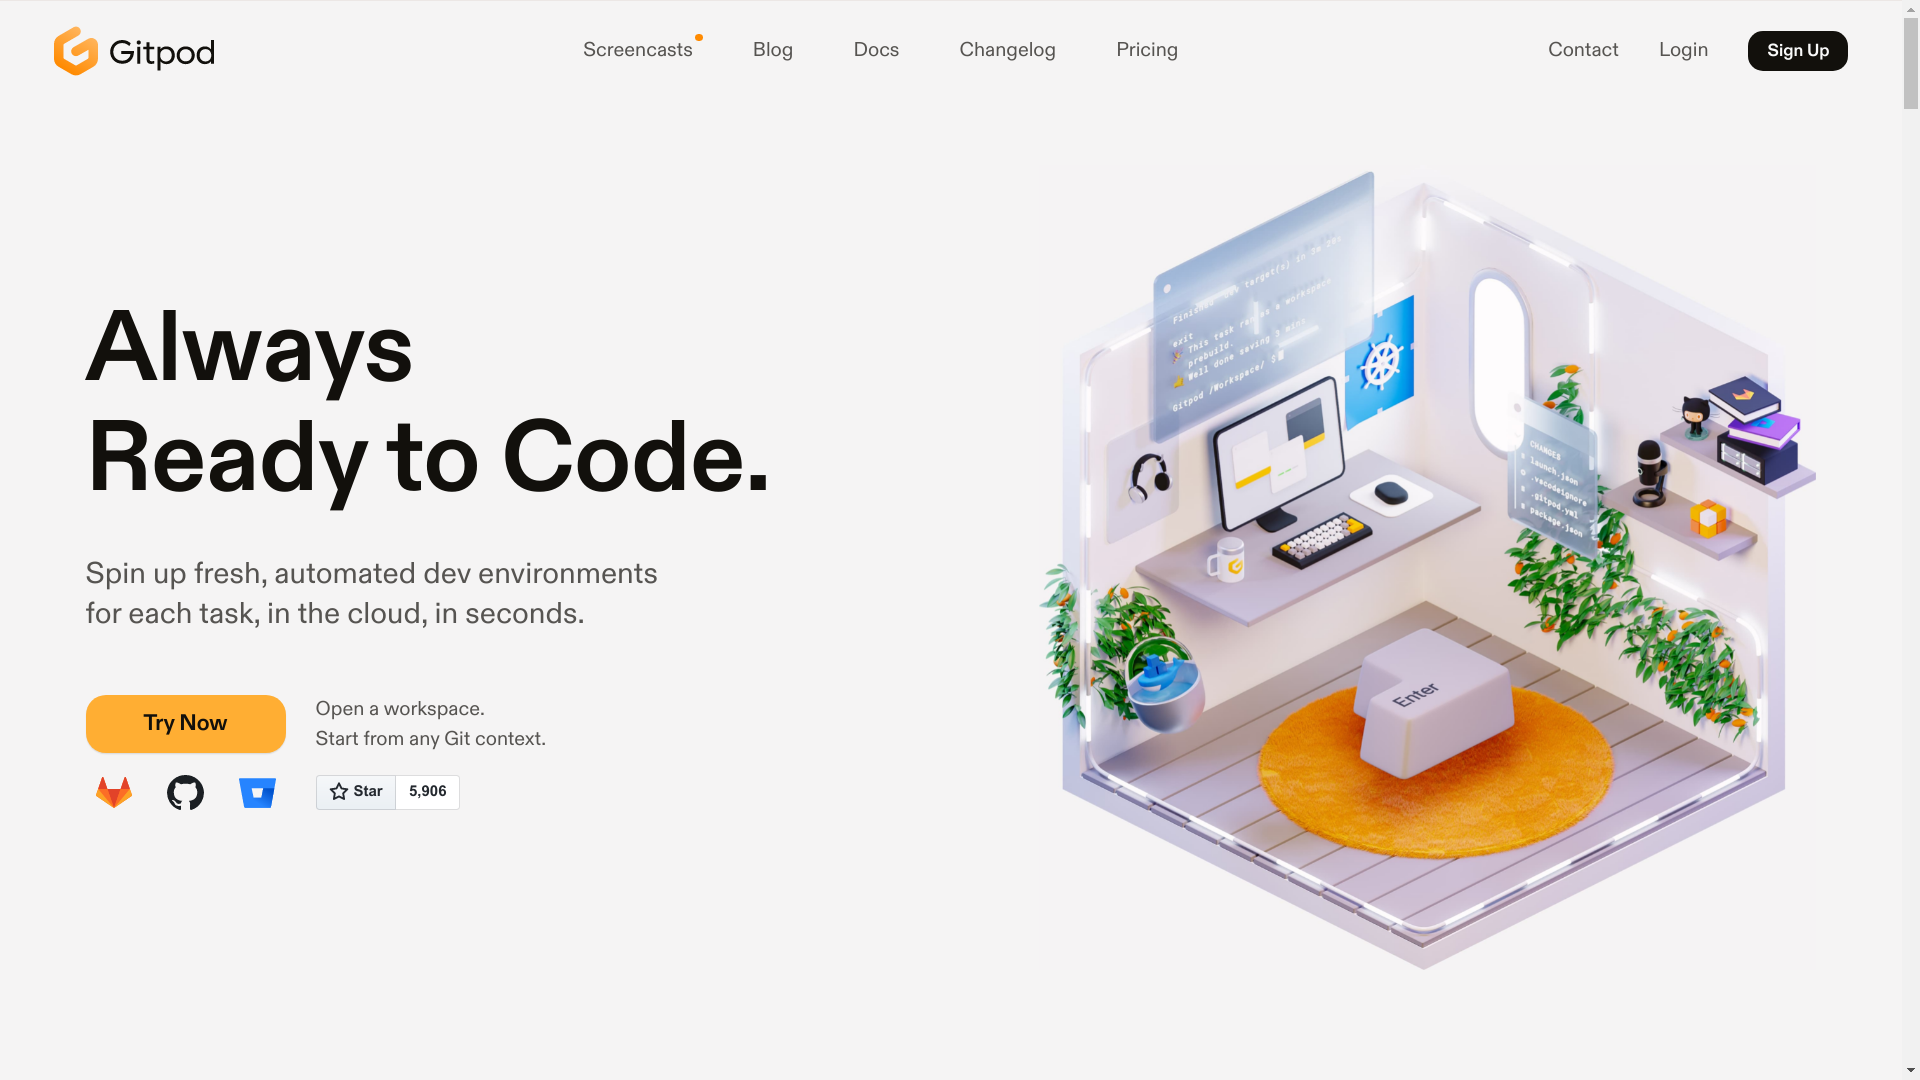
\includegraphics[width=.6\paperwidth]{images/homepage}
	      \end{figure}

	\item \url{https://gitpod.io/#https://github.com/cpp-review-dune/dune-book}
	      \begin{figure}[ht!]
		      \centering
		      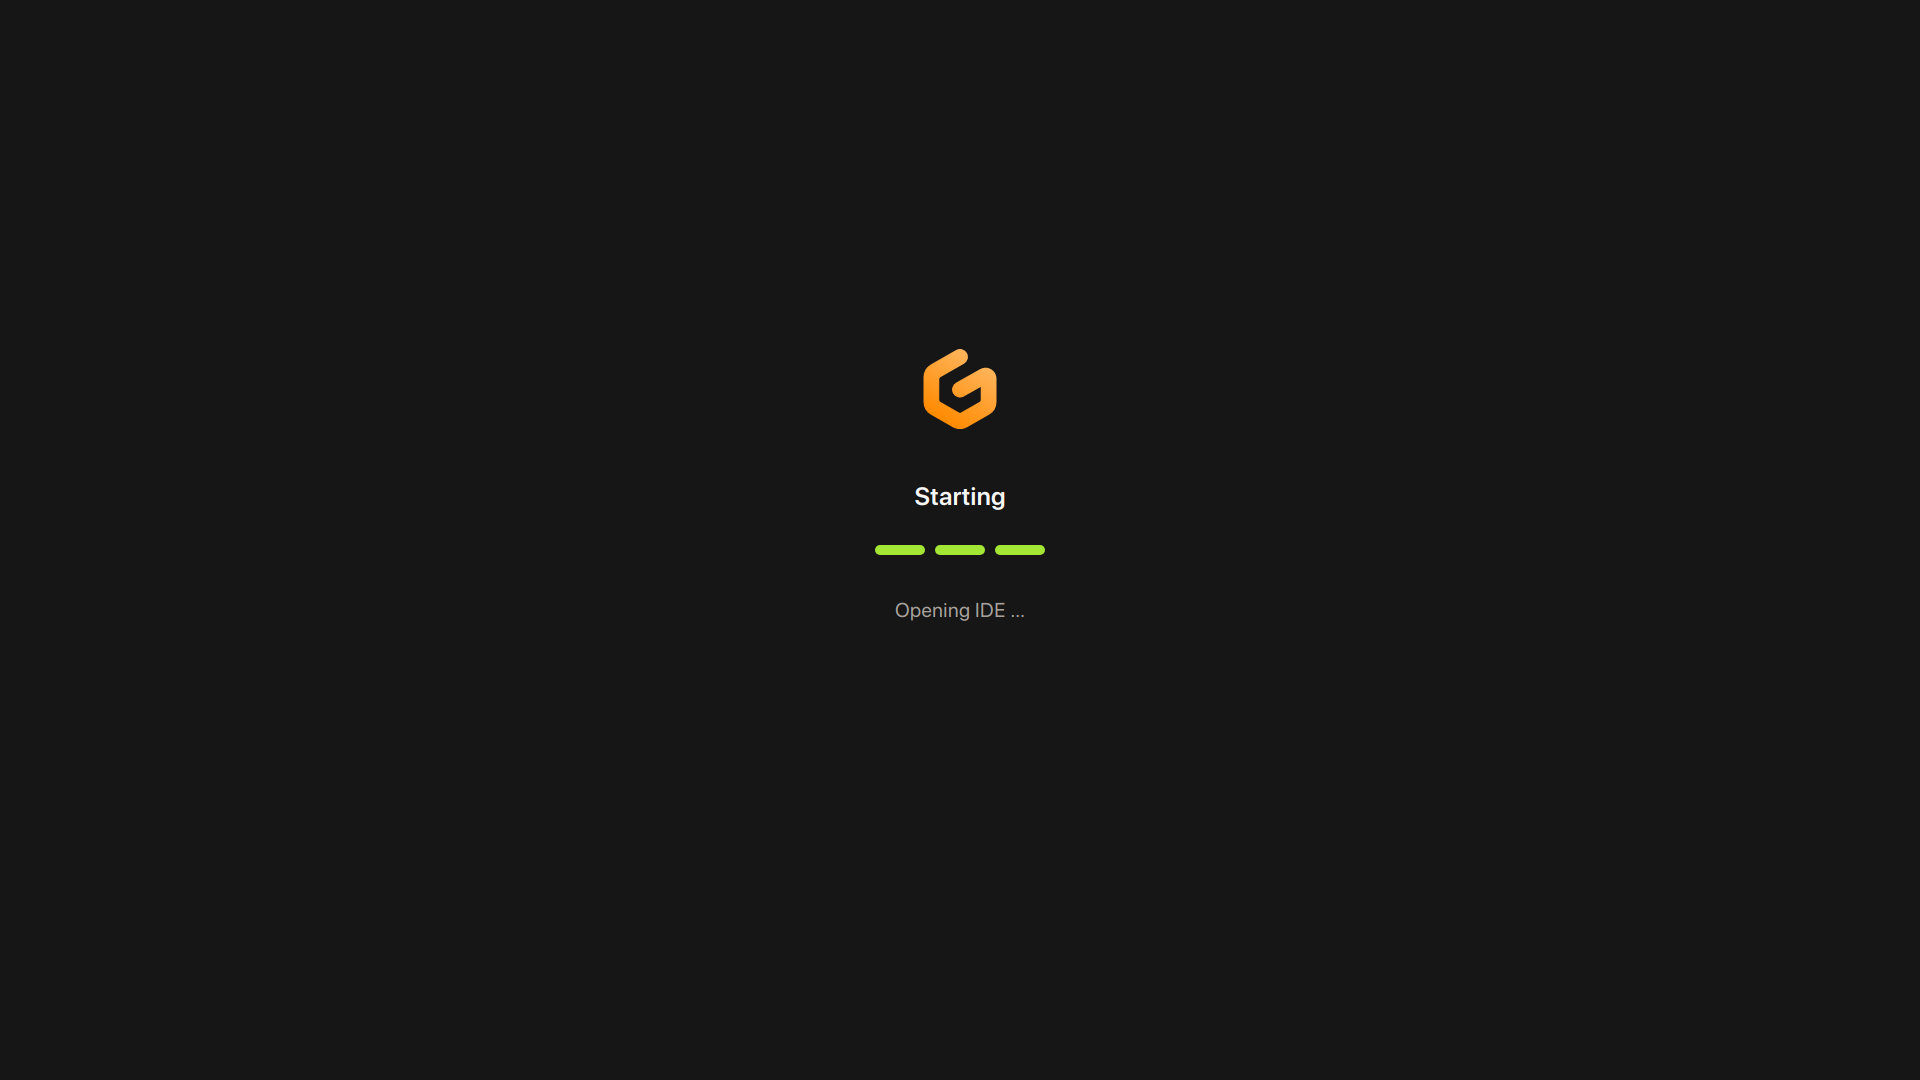
\includegraphics[width=.6\paperwidth]{images/opening}
	      \end{figure}
	      \begin{figure}[ht!]
		      \centering
		      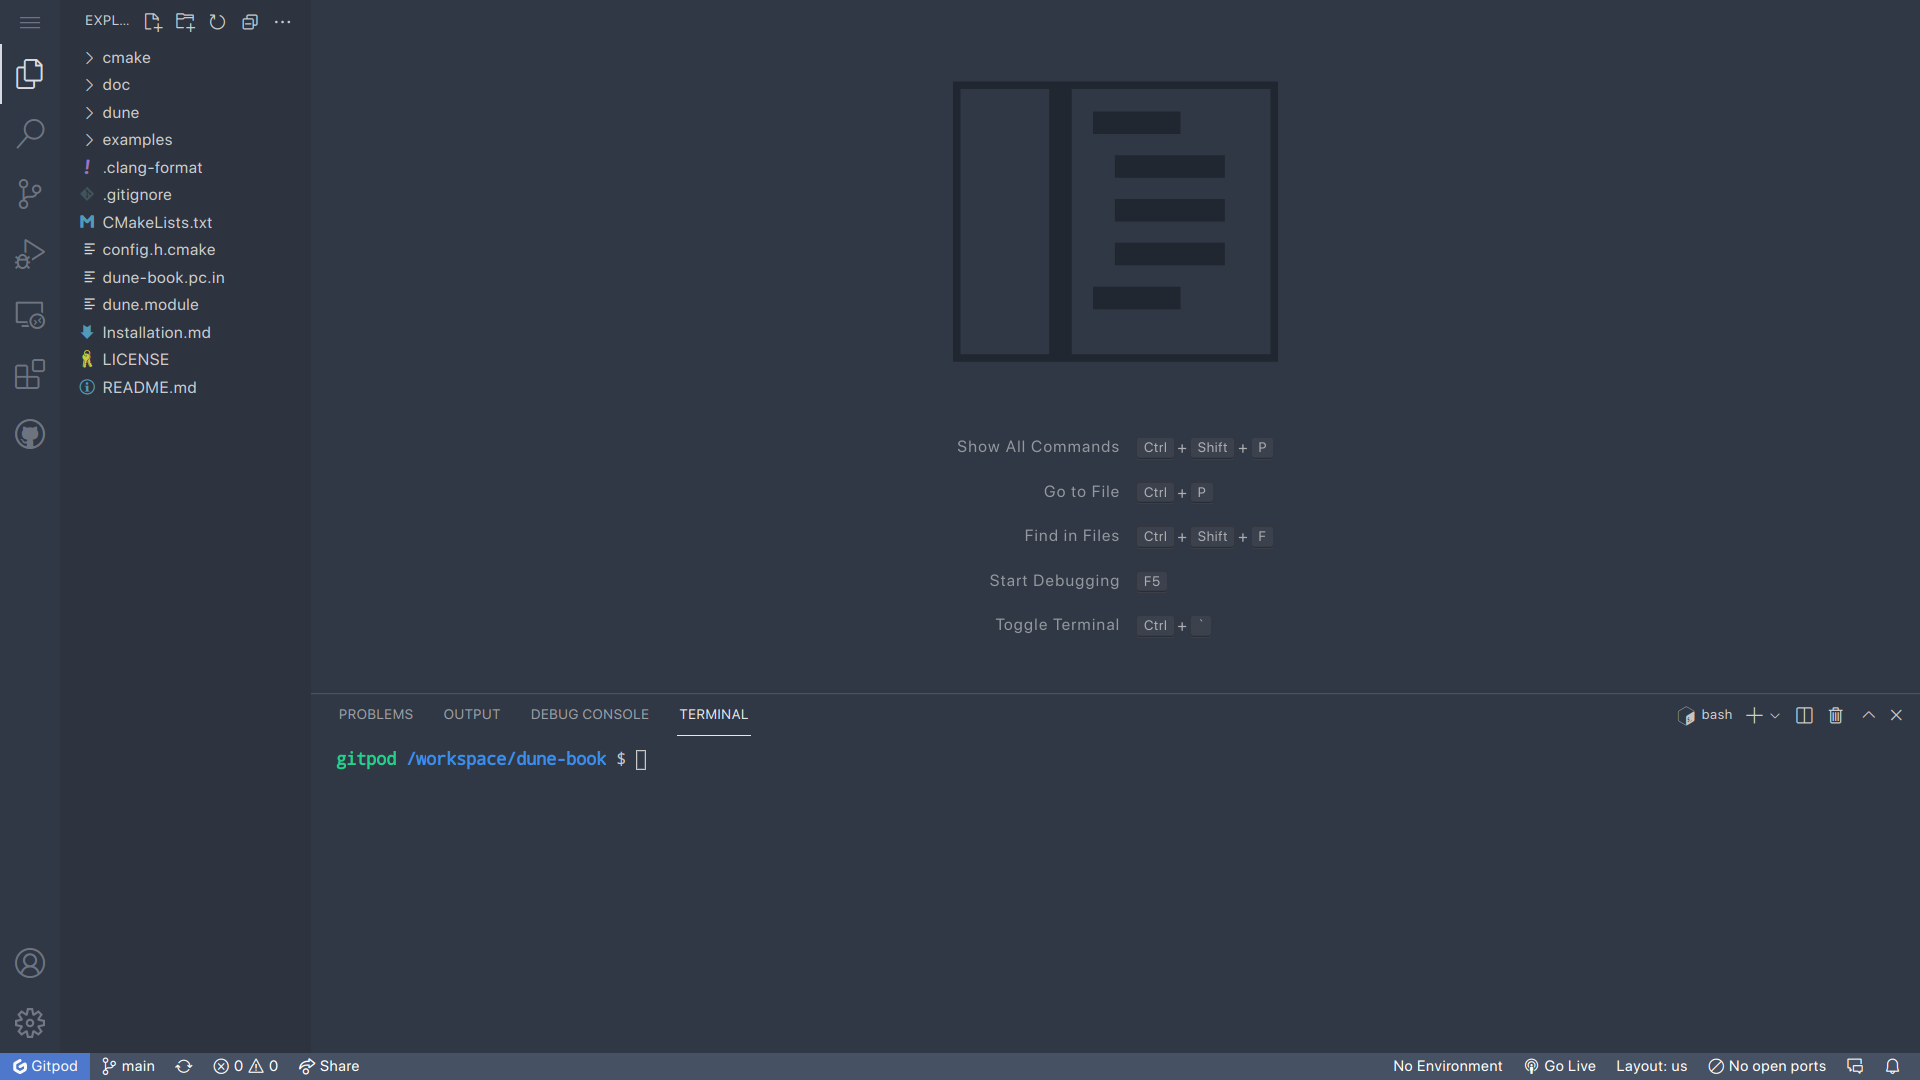
\includegraphics[width=.6\paperwidth]{images/editor}
	      \end{figure}
	      \begin{figure}[ht!]
		      \centering
		      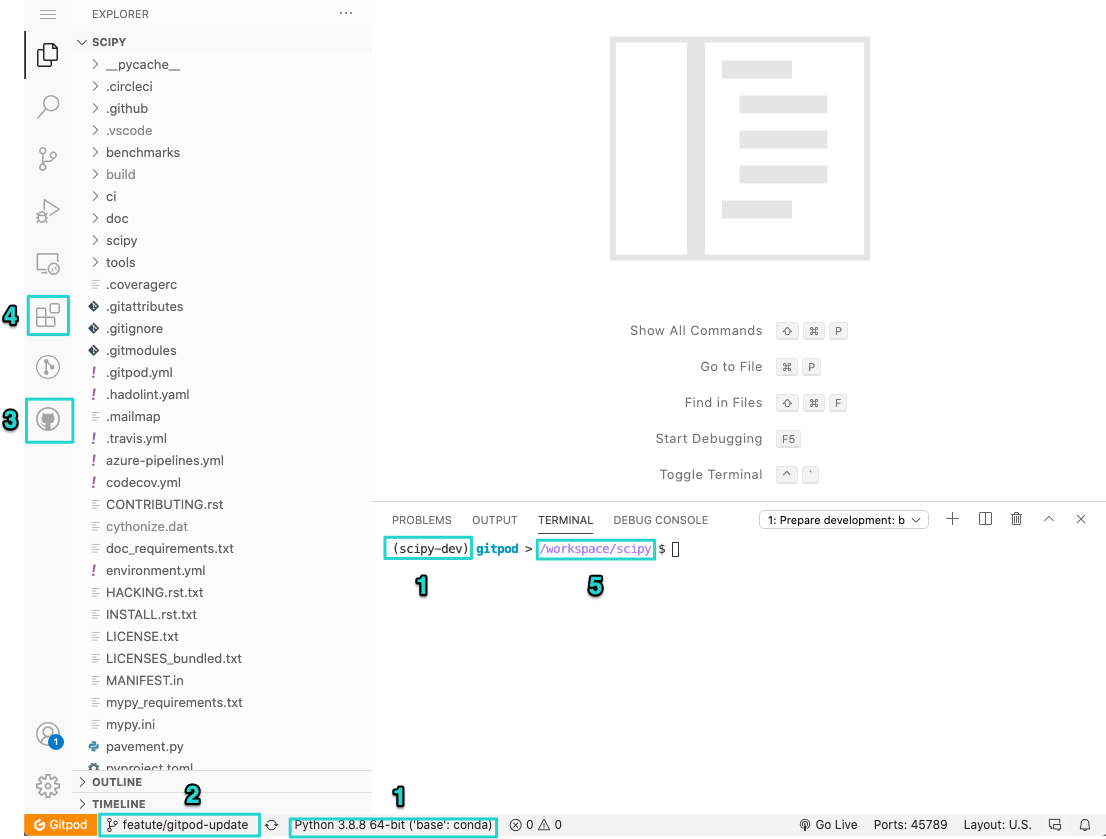
\includegraphics[width=.6\paperwidth]{images/gitpod-workspace}
		      \caption{Imagen de referencia.}
	      \end{figure}
        \item Crear un archivo, usar la terminal, crear carpetas, cambiar el tamaño de la letra (archivos/preferencias/configuración).
        \item Ejecute un programa en python, construya un proyecto en cmake.
        \item Cerrar el espacio de trabajo
	      % https://scipy.github.io/devdocs/dev/contributor/quickstart_gitpod.html
\end{enumerate}

\section{GitHub}

Para darse de alta en GitHub, necesitará completar el formulario \url{https://github.com/signup} y seguir la ayuda en línea \url{https://docs.github.com/es/get-started/quickstart} para configurar la herramienta git, crear repositorios, flujos de trabajo cooperativos.

\begin{figure}[ht!]
	\centering
	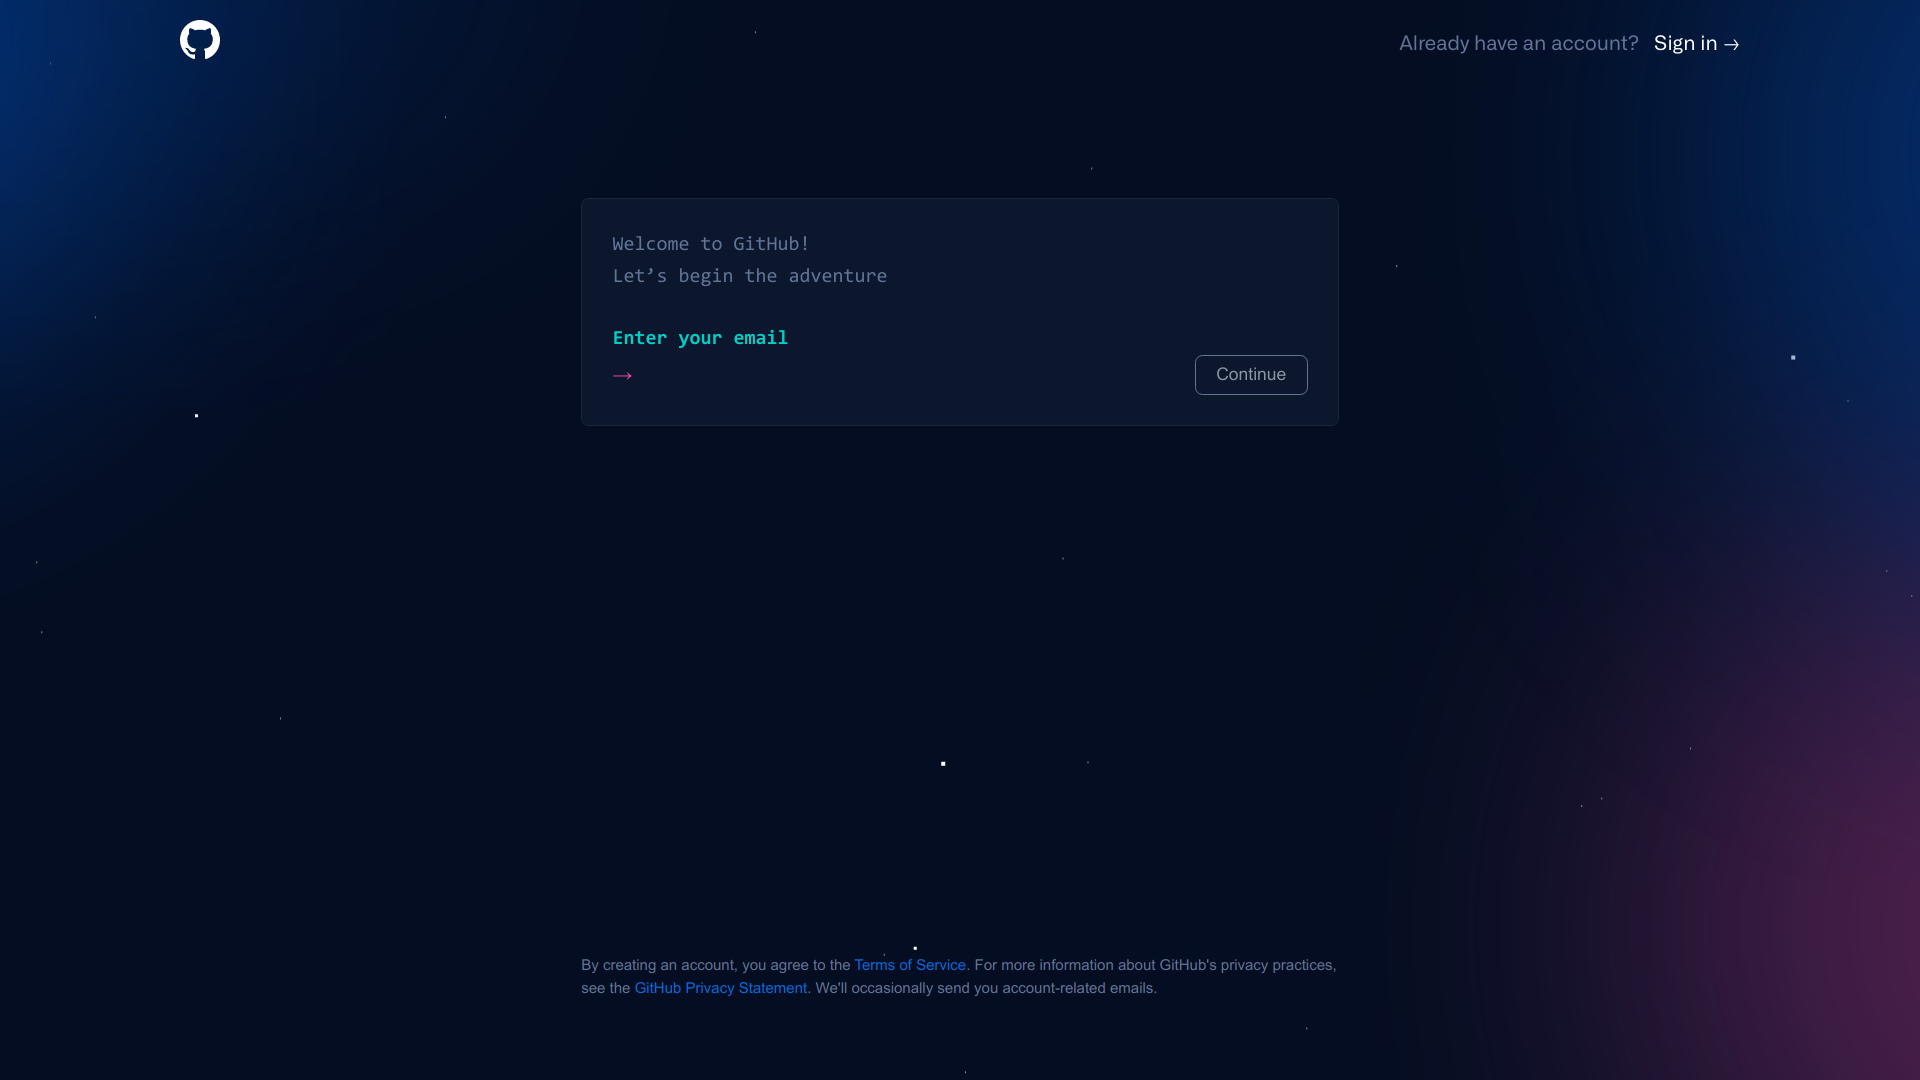
\includegraphics[width=.6\paperwidth]{images/signup}
\end{figure}



\section{GNU/Linux}

\subsection{Docker}

\url{https://docs.microsoft.com/es-es/dotnet/architecture/containerized-lifecycle/docker-terminology}

\begin{quote}
	Docker es un proyecto de código abierto para automatizar la implementación de aplicaciones como contenedores portátiles y autosuficientes que se pueden ejecutar en la nube o localmente.
	% \ref{msdocker}
	% TODO: Citar https://docs.microsoft.com/es-es/dotnet/architecture/containerized-lifecycle/what-is-docker
\end{quote}

\subsubsection{\texttt{docker run}}

\url{https://docs.docker.com/engine/reference/commandline/run}
\url{https://docs.docker.com/engine/reference/commandline/images}
\url{https://docs.docker.com/engine/reference/commandline/exec}

% Ejemplos

\begin{enumerate}
	\item Nos dirigiremos a \url{https://github.com/orgs/cpp-review-dune/packages} y seleccionaremos la imagen docker \texttt{dunepdelab}.
	      \begin{figure}[ht!]
		      \centering
		      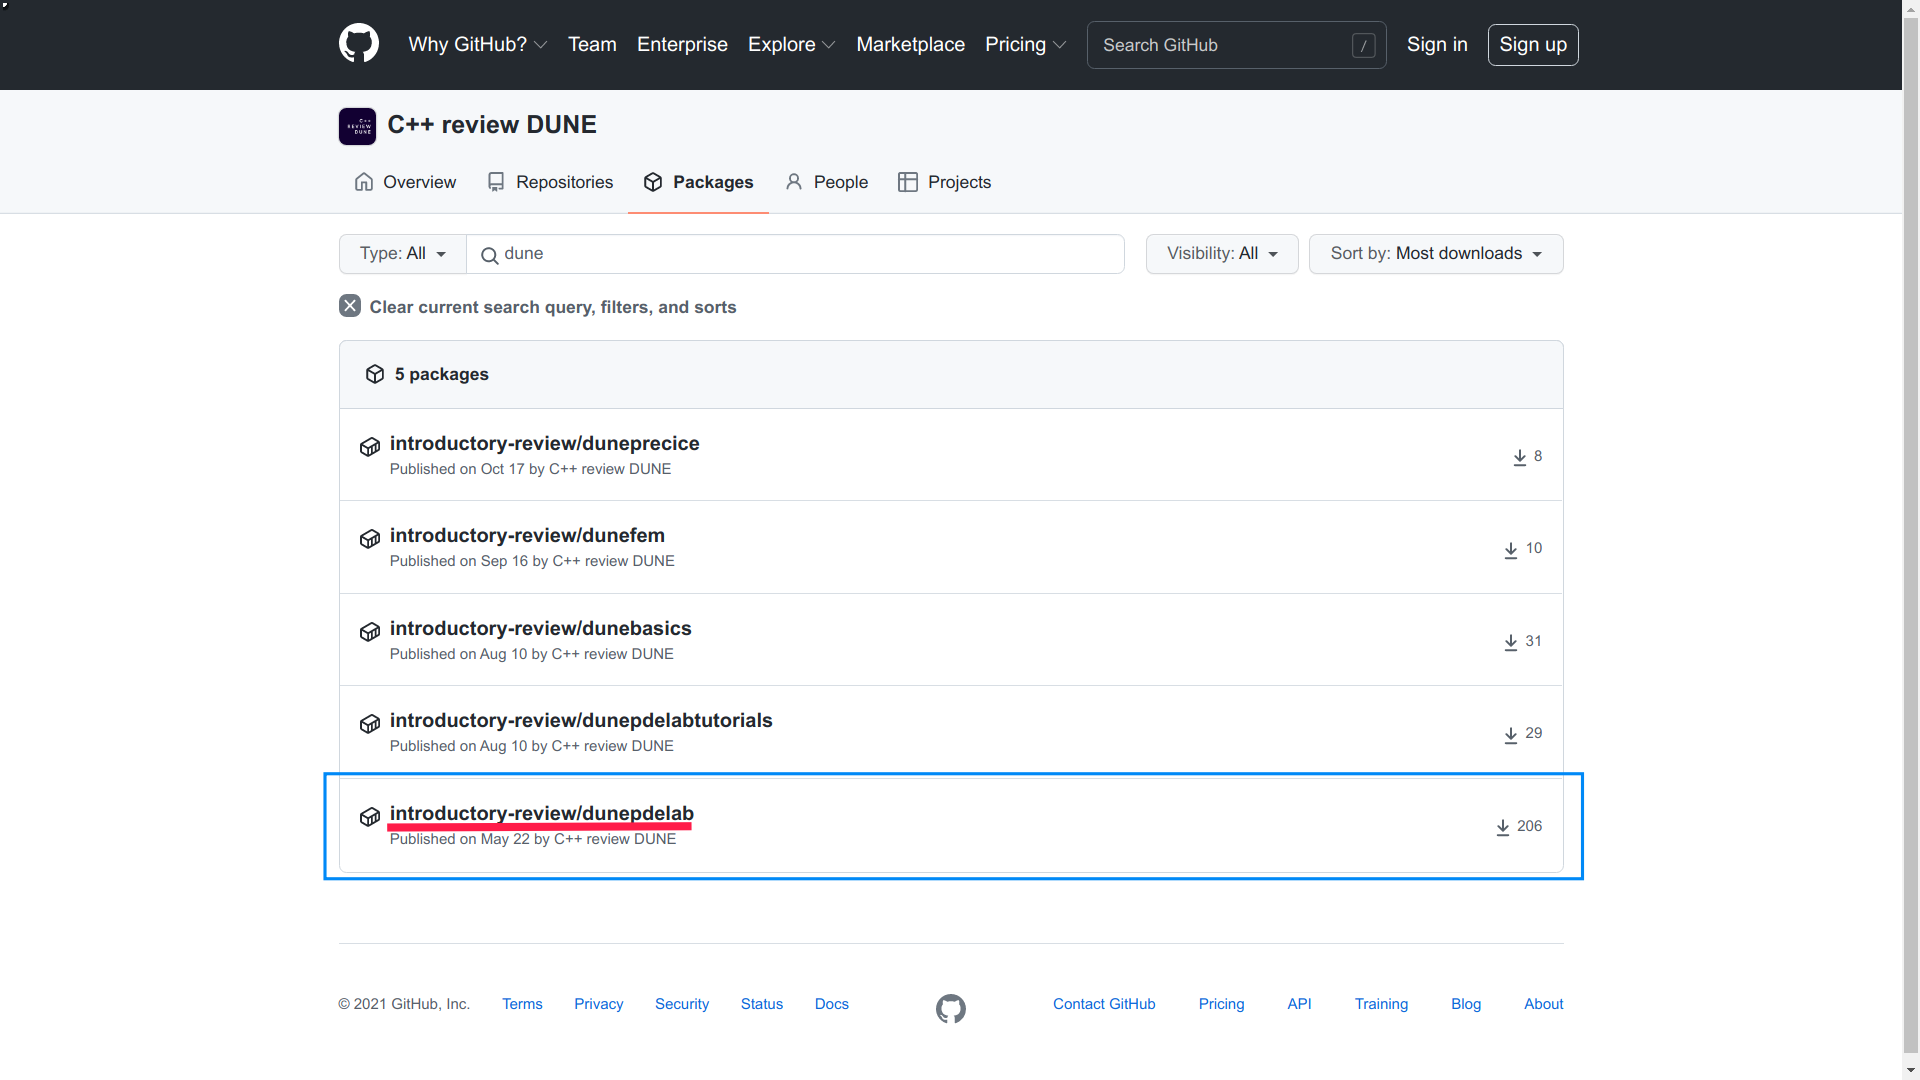
\includegraphics[width=.6\paperwidth]{images/imagedunepdelab}
	      \end{figure}
\end{enumerate}

\subsection{Debian based, Arch based}

% En caso que Gitpod soporte Arch, no mencionaré Ubuntu.

\section{Arch Linux}

% TODO: Errores frecuentes

Los principios de Arch Linux
% https://wiki.archlinux.org/title/Arch_Linux_(Espa%C3%B1ol)#Principios

Las diferencias entre Arch Linux y las demás.
% 1 párrafo
para los usuarios que ya han usado Linux pueden ver \url{https://wiki.archlinux.org/title/Pacman_(Espa%C3%B1ol)/Rosetta_(Espa%C3%B1ol)}
% https://wiki.archlinux.org/title/Arch_compared_to_other_distributions_(Espa%C3%B1ol)

Mostrar ejemplos, cómo se actualiza, cómo se instala, cómo se busca.

% Clonar, cambiar las ramas, subir y bajar los cambios.
	\chapter{Modelos con EDO y EDP}
	Presentar una serie de ejemplos y ejercicios clásicos, con sus descripciones
caracaterísticas, condiciones iniciales o de frontera.  Una selección 
de teorías, partiendo por ejemplo de las leyes de conservación y de las 
leyes empíricas, Ley de Fourier, Ley de Darcy, Leyes de Maxwell, Leyes 
en el tránsito, flujos en suelos y plantas, circuitos.
Ecuación de Poisson, Ecuación de Onda, etc.

Es importante la explicación de la condiciones de frontera tipo Dirichlet y Neuman.
Posiblemente, en los libros de Heildeberg. También revisar el libro del profesor 
Hernán Estrada.

\section{La derivada}
El modelamiento matemático es una técnica que utilizan principalmente los matemáticos e ingenieros 
para comprender, simular y predecir el comportamiento de sistemas físicos.  Newton fue uno de 
los precursores, buscaba predecir el comportamiento de los cuerpos que se movían, por ejemplo
tratar de explicar la rotación de los planetas alrededor del sol, o un coche que se moviera en una 
dirección particular.  Para tratar de comprender lo que ocurría, inventó algunos conceptos que son 
muy utilizados hoy en día, por ejemplo el concepto de fuerza, y a diferencia de lo que se había planteado
anteriormente, Newton estableció que todo cuerpo tiende a mantener su estado, excepto que haya una
fuerza externa que cambié su estado inicial.  

Estableció entonces tres leyes que rigen los movimientos de los cuerpos, a saber:

\section{Leyes de conservación}
En primer lugar nos vamos a referir a un \textit{sistema cerrado}, que corresponde a una región 
del espacio que tiene fronteras en el cual siempre se conserva alguna cantidad particular, a la cual
le podemos dar una representación numérica.  Para empezar vamos a determinar la ecuación 
de conservación unidimensional de la masa de un gas en un cilindro. El gas fluye en el tubo en la 
dirección positiva de las $x$, tanto la densidad como la velocidad del gas se suponen constantes cuando
cruzan la sección transversal del cilindro como se aprecia en la figura \ref{fig:cilindro01}. La densidad
se define de tal forma que la masa total $u(x,t)$ del gas en algun intervalo dado $\left[a,b\right]$ 
por ejemplo, está dada por la integral de la densidad como en la ecuación \eqref{eq:masatotal01}:
\begin{equation}\label{eq:masatotal01}
u(x,t)=\int_{a}^{b} \rho(x,t)dx
\end{equation}

\begin{figure}\label{fig:cilindro01}
    \centering
    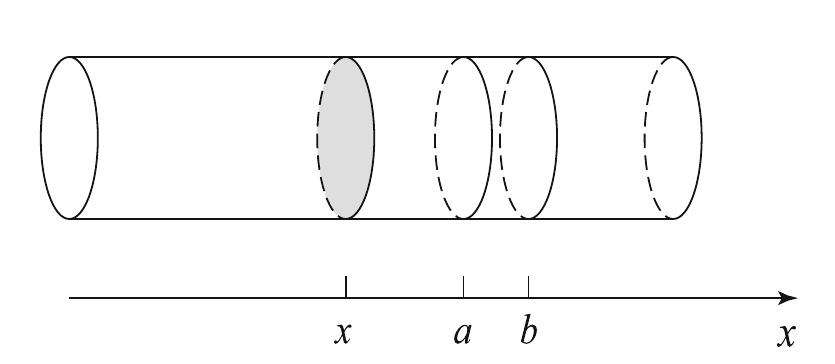
\includegraphics[scale=0.5]{images/cilindro01}
    \caption{Cilindro en el que fluye una masa de gas, en x hay una sección transversal}
\end{figure}

Si suponemos que las paredes del cilindro son impermeables, y la masa del gas ni se crea ni se destruye
al interior del cilindro, entonces la masa en ésta sección sólo puede cambiar debido al flujo del gas
del punto $a$ al punto $b$.

Ahora, supongamos que $v(x,t)$ es la velocidad del gas en el punto $x$ al tiempo $t$.  Entonces la 
velocidad del flujo o el flujo másico $\phi$ que pasa por éste punto estará dado por la ecuación 
\eqref{eq:flujo-masico}:
\begin{equation}\label{eq:flujo-masico}
    \phi(x,t) = \rho(x,t)v(x,t)
\end{equation}
Que al establecer las unidades resulta en la expresión \eqref{eq:unidades01}:
\begin{equation}\label{eq:unidades01}
    \left[\phi\right]=\frac{kg}{s} = \left[\rho\right]\left[v\right]= \frac{kg}{\cancel{cm}}\frac{\cancel{cm}}{s}
\end{equation}

Así el flujo másico tendrá unidades de kilogramos ''$kg$'' por segundo ''$s$'', es decir una medida de la 
cantidad de masa que pasa por cada segundo en un $x$ particular.

Debido a que el flujo másico tiene unidades de kilogramos por segundo, entonces podemos derivar la 
ecuación \eqref{eq:masatotal01} de donde obtenemos la razón de cambio de la masa en el intervalo
$[a,b]$ por la expresión \eqref{eq:cambio_masa}:
\begin{equation}\label{eq:cambio_masa}
    \frac{d u(x,t)}{dt} = \frac{d}{dt}\int_a^b\rho(x,t)dx=\overbrace{\rho(a,t)v(a,t)}^{masa\ que\ entra}
    -\underbrace{\rho(b,t)v(b,t)}_{masa\ que\ sale}
\end{equation}
Que se puede interpretar como, el cambio en la masa en un instante de tiempo, es igual a la cantidad 
de masa que entra en el intervalo, menos la cantidad de masa que sale. La ecuación \eqref{eq:cambio_masa}
es una forma \textbf{integral} de la ley de conservación.
\section{Casos especiales de las leyes de conservación}

\section{Ejemplos de modelos matemáticos}


\section{Aplicaciones}
\subsection{Ecuación de Poisson}
\subsection{Otras aplicaciones}
	\chapter{Elementos Finitos}
	Una revisión básica de los conceptos presentados en el curso de 
DUNEPDELab, las presentaciones de Peter Bastian, explicando los 
enmallados, las numeraciones, los recorridos, los tipos de elementos.

	\chapter{Mallas y Software}
	Se escribiría la explicación teórica y el uso del software gmsh, estan los de python.

% Recursos:
% https://github.com/cpp-review-dune/dune-basics/blob/13bb9abcb3c7c2591a982f22f8a1288ad770b189/dune-basics/doc/beamer/dune-gmsh.tex#L180
% https://bthierry.pages.math.cnrs.fr/tutorial/gmsh/
% https://www.youtube.com/watch?v=aFc6Wpm69xo

Se puede hacer la presentación de GMSH, introducción básica, creación de figuras, puntos, líneas, curvas y superficies.


	\chapter{Algorítmos y Programación DUNE C++}
	\section{Historia de DUNE}

% Fechas de lanzamientos, nos encontramos en Dune.

\section{Filosofía del programa}

\section{Estructura de DUNE}
\section{DUMUX, Y OTROS SOFTWARE BASADOS EN DUNE} % Precice

Un ejemplo interesante puede ser parecido a:

\url{https://gitlab.com/tobias.kies}

\section{Versiones}

% https://dune-project.org/releases/2.8.0/

\begin{table}[ht!]
	\centering
	\begin{tabular}{|c|c|c|c|}
		\hline
		Nombre de la función/plantilla
		 &
		Descripción
		 &
		¿Compatible con la versión 2.8.X?
		 &
		Ejemplo   \\
		\hline
		 &   &  & \\
		\hline
	\end{tabular}
\end{table}

\section{Dune FEM y PDElab}
	\chapter{Algorítmos y Programación DUNE Python}
	Se haga un desarrollo similar a lo que sucede en cpp
	\chapter{Herramientas Complementarias}
	\section{Yaml y Docker}
	En ésta parte del documento, se debe documentar el uso de la imagen
archiso para ser utilizada en un virtualbox, o para ser utilizada
en gitpod.

También se pueden hacer las descripciones del manejo en jupyternotebook
	\section{Doxygen}
	Dada una función o una clase de plantilla en c++ documentar los parámetros, explicar los pasos, como se inicializa,
como se genera la documentación en html y latex.
	\section{Markdown}
	Mostrar los aspectos más sobresalientes para presentar la documentación.
	\section{Paraview y Gnuplot}
	Se busca hacer una introducción muy básica pero eficiente del manejo de paraview, cargar datos,
hacer la simulación, exportar gráficos y vtu, visualizar animaciones, etc. 

Gnuplot, también es una introducción al manejo de datos desde archivos, un poco de formato y
tipos de salidas.
	
	

	
	B.\cite{Reilly}

	\printbibliography[
	title={Referencias},
	heading=bibintoc]
	% TODO Poner correctamente la bibliografía y referencia: ver https://tex.stackexchange.com/a/183274/117967
	\nocite{*}
	\printbibliography[
	title={Bibliografía},
	heading=none,keyword=paper]
\end{refsection}

A\index{A}.

$$\int_a^b f(x)dx$$

Probando la llave ssh, probando el repositorio en github

\printindex

\end{document}

